Magnetische Felder werden durch bewegte elektrische Ladungen erzeugt.
Das Magnetfeld lässt sich durch die magnetische Feldstärke $\vec{H}$ und die magnetische Flussdichte $\vec{B}$ beschreiben.
$\vec{H}$ beschreibt den Betrag und die Richtung des Magnetfelds.
$\vec{B}$ nimmt außerdem die magnetische Permeabilität $\mu=\mu_{0}\cdot\mu_{r}$ in die Betrachtung mit auf.
$\mu_{0}=\SI{4\pi e-07}{\frac{VS}{Am}}$ ist dabei die Vakuum-Permeabilität oder auch magnetische Feldkonstante.
$\mu_{r}$ ist die materialabhängige Permeabilität.
\\Für die beiden vektoriellen Größen $\vec{H}$ und $\vec{B}$ gilt folgender Zusammenhang:
\begin{equation*}
  \vec{B}= \mu_{0} \cdot \mu_{r} \cdot \vec{H}.
\end{equation*}
\\Bewegte Ladungen kommen in stromdurchflossenen Leitern vor, entsprechend entsteht um einen solchen Leiter ein Magnetfeld.
Über das Biot-Savart'sche Gesetz
\begin{equation*}
  \vec{B}(\vec{r})= \frac{\mu_{0}I}{4 \pi} \int_{\symup{Leiter}} \! \frac{d\vec{l} \times (\vec{r}-\vec{r'})}{|\vec{r}-\vec{r'}|^3}
\end{equation*}
\\mit dem Strom I und dem infinitesimalen Leiterstück $d\vec{l}$ lässt sich im Abstand $\vec{r'}-\vec{r}$ die magnetische Flussdichte berechnen.
\\Für eine lange Spule der Länge l und der Windungszahl N ergibt sich der Betrag der magnetischen Flussdichte zu
\begin{equation}
  B= \mu_{0} \mu_{r} \frac{N I}{l}.
  \label{eqn:ls}
\end{equation}
\\Das Magnetfeld innerhalb einer langen Spule ist näherungsweise homogen und wird zu den Enden der Spule inhomogen.
\\Eine Toroidspule mit dem Radius R hat die magnetische Flussdichte
\begin{equation*}
  B= \mu_{0} \mu_{r} \frac{N I}{2 \pi R}.
\end{equation*}
\\In der Toroidspule ist das Magnetfeld homogen, außerhalb ist kein Magnetfeld vorhanden.
\\Für ein Paar Helmholtzspulen mit dem Radius R und mit dem Abstand x zum Mittelpunkt gilt im Mittelpunkt zwischen den beiden Spulen folgende Gleichung:
\begin{equation}
  B(0)= \mu_{0} \frac{N I R^2}{ \left(R^2 + x^2 \right)^{3/2}}.
  \label{eqn:helm}
\end{equation}
\\Für ideale Helmholtzspulen ist der Abstand der Spulen gleich dem Radius der Spulen.
Da dies nicht immer der Fall ist, wird der allgemeine Fall berechnet.
\\Ferromagnetische Materialien haben eine sehr große relative Permeabilität $\mu_{r}$.
Dabei gilt folgende Beziehnung nicht mehr:
\begin{equation*}
    \vec{B}= \mu_{r} \cdot \vec{H}.
\end{equation*}
\begin{figure}
  \centering
  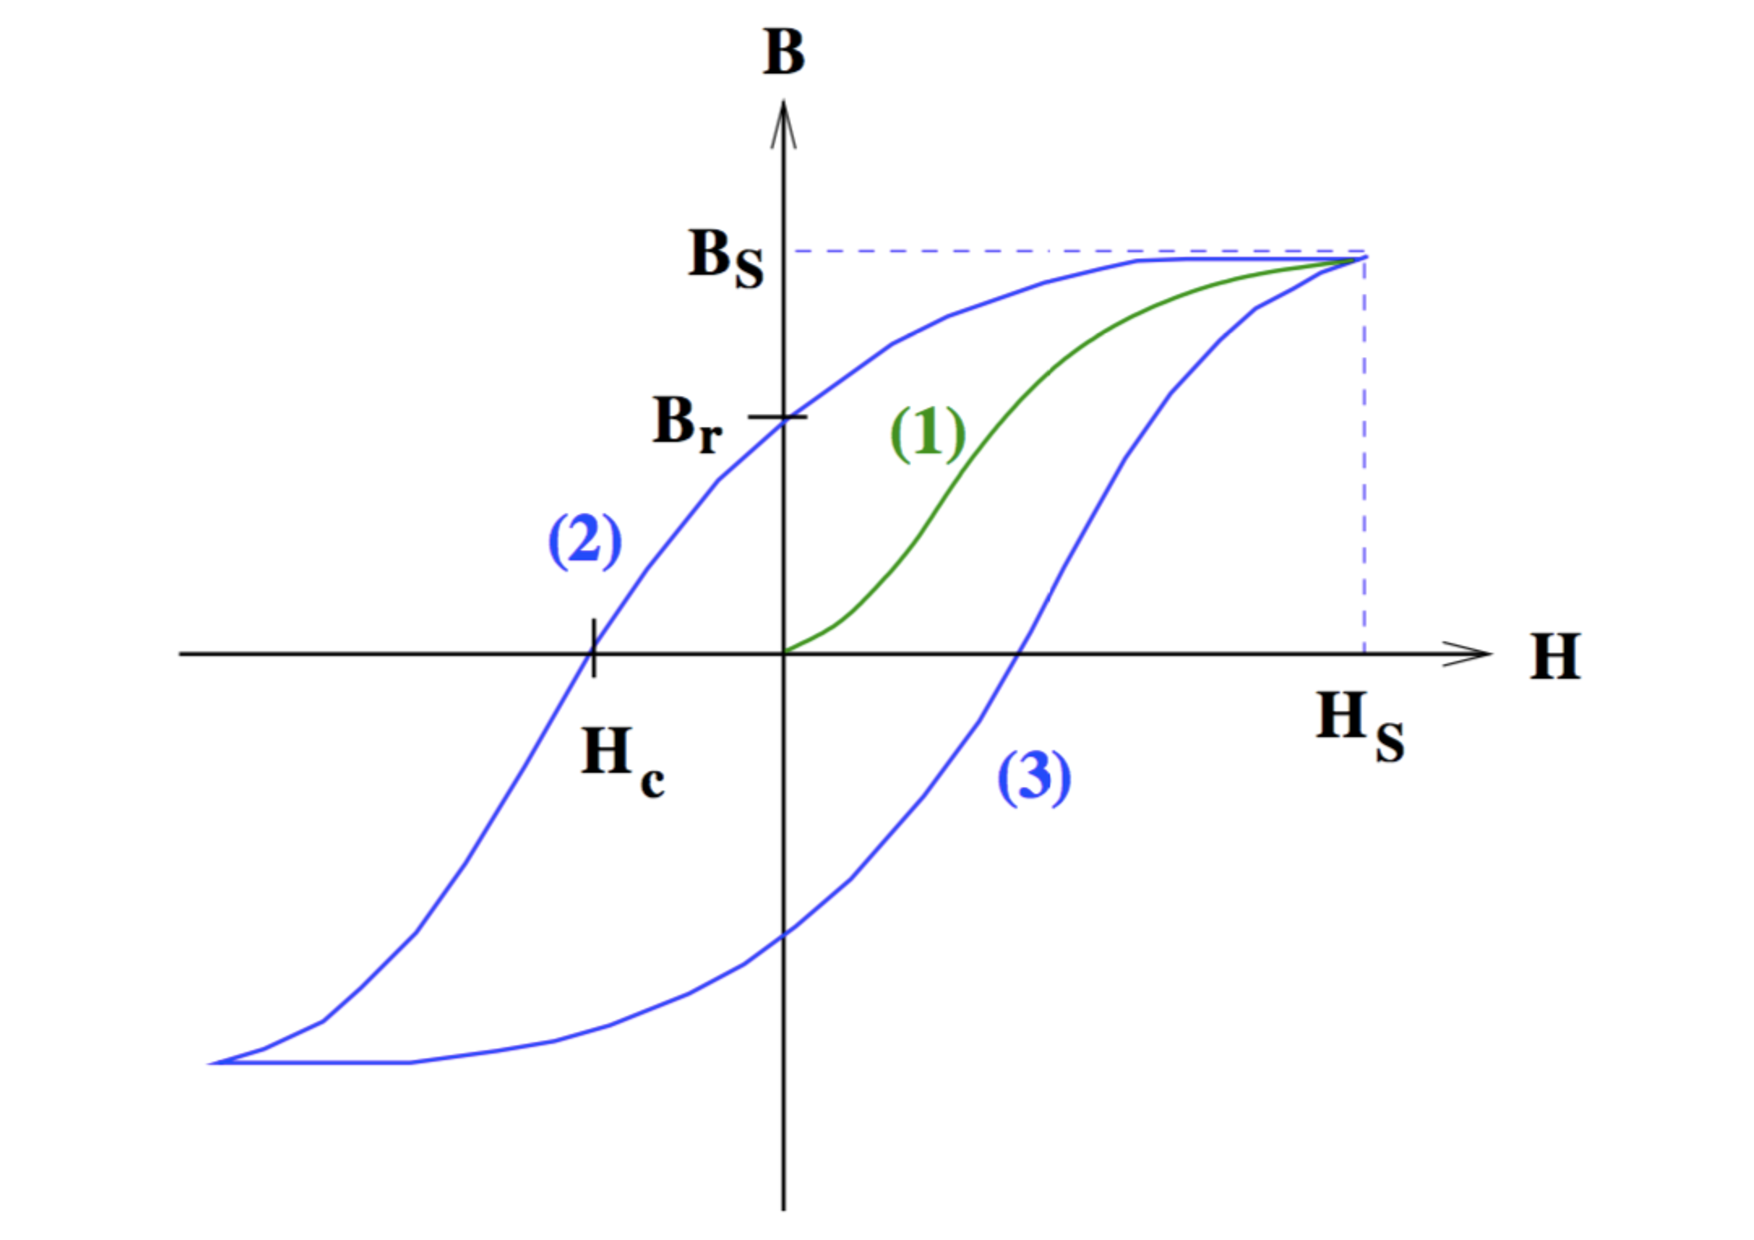
\includegraphics[width=\textwidth]{hys.pdf}
  \caption{Hysteresekurve \cite{1}}
  \label{fig:hys}
\end{figure}
\\Die relative Permeabilität ist also eine Funktion der magnetischen Feldstärke $\vec{H}$.
\\Ferromagnetische Materialien haben auch ohne äußeres Magnetfeld ein permanentes magnetisches Moment.
Innerhalb der Weiß'schen Bezirke ist das magnetische Moment gleich, über das Material sind die Weiß'schen Bezirke statistisch in alle Richtungen ausgerichtet und führen so dazu, dass das Material kein eigenes Magnetfeld hat.
Ein äußeres Magnetfeld richtet die magnetischen Momente aus und das Material bewirkt eine Verstärkung des Magnetfelds.
Außerdem wird das Material zunehmend magnetisiert, da sich die magnetischen Momente nicht alle wieder in alle Richtungen ausrichten.
Dieses Verhalten lässt sich durch eine Hysteresekurve (Abbildung \ref{fig:hys}) darstellen.
\\Wird der Strom in der Spule hochgeregelt, steigt zunächst das B-Feld auf den Sättigungswert $B_{s}$.
Wird der Spulenstrom runtergeregelt, fällt das B-Feld dann mit einer anderen Steigung auf den negativen Sättigungswert.
\\Der Schnittpunkt $B_{r}$ mit der B-Achse wird Remanenz genannt. Diese beschreibt die Restmagnetisierung im Material, die ohne äußeres Feld wirkt.
\\Die Nullstelle $H_{c}$ dieser Kurve wird Koerzitivkraft genannt. Die Koerzitivkraft ist der Wert, um den das B-Feld erhöht werden muss damit im Material die Restmagnetisierung ausgeglichen ist.
\\Wird der Spulenstrom nun wieder erhöht, verläuft die Kurve ähnlich, aber verschoben zum Sättigungswert.
